\documentclass[12pt, a4paper,oneside]{book}
% Подключение библиотеки
\usepackage{/Users/vladbelousov/Desktop/Semestr_4-FP-NSU/Настройка/library}

\begin{document}

\begin{titlepage}
    \thispagestyle{empty}  % Отключаем нумерацию страницы на титульном листе
    \centering
    \vspace*{1cm}  % Отступ сверху

    \textbf{\huge Конспект лекций по дисциплине}  \\[1.5cm]  % Название
    \textbf{\huge Основы функционального анализа}  \\[2cm]   % Название дисциплины (оставьте пустым для добавления вручную)
    \textbf{\Large Новосибирский государственный университет} \\[0.5cm]
    \textbf{\large Физический факультет} \\[0.5cm]
    \textbf{\large 4-й семестр} \\[0.5cm]
    \textbf{\large 2025 год} \\[10cm]

    \begin{flushright}
        \large Студент: Б.В.О \\[0.5cm]  % Ваше имя
        Преподаватель: Ротанова Татьяна Александровна  % Ф.И.О. преподавателя
    \end{flushright}
\end{titlepage}

\tableofcontents  % Создание оглавления

\def\mainfile{}  % Определяем макрос для основного файла
% Условная компиляция для самостоятельной работы
\ifdefined\mainfile
    % Если это часть основного файла, не добавляем начало и конец документа
\else
    \documentclass[12pt, a4paper]{report}
    \usepackage{/Users/vladbelousov/Desktop/Semestr_4-FP-NSU/Настройка/library}
    \usepackage[utf8]{inputenc} % Подключение поддержки UTF-8
    \begin{document}
\fi

%%-------------------------------%%

\chapter{Геометрия пространств со скалярным произведением.}

\begin{center}
    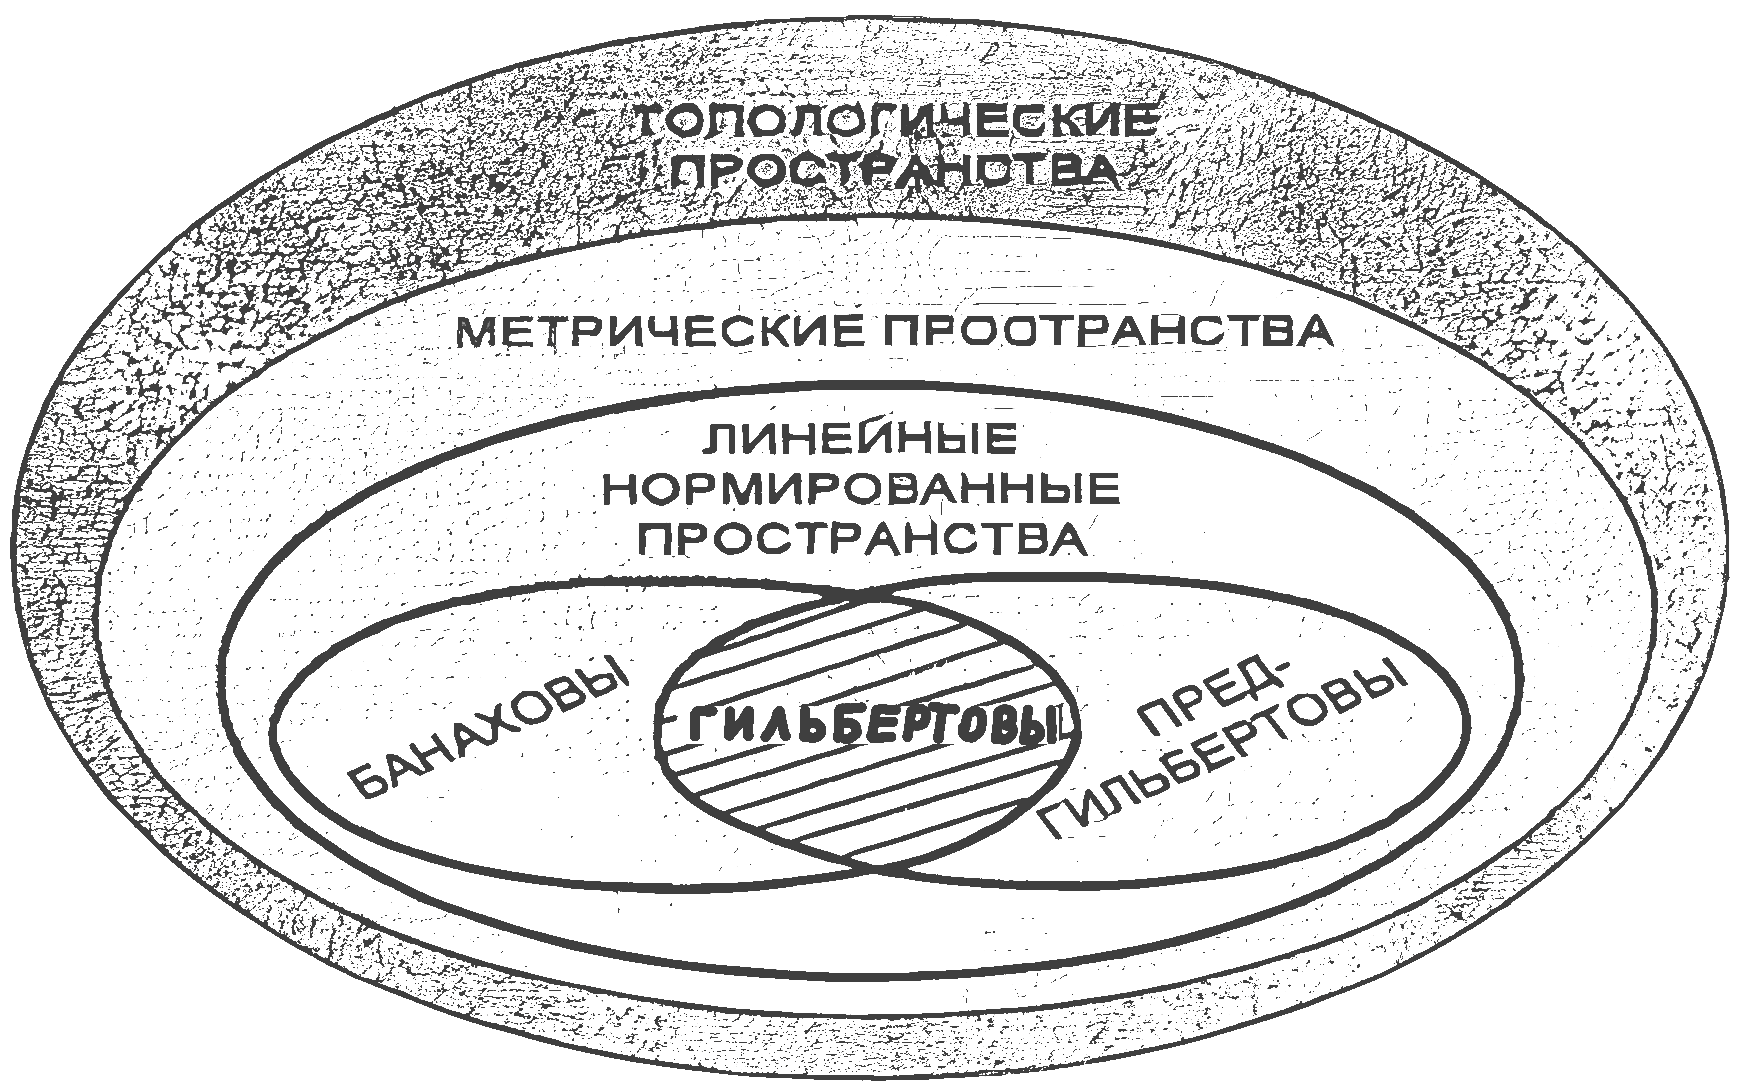
\includegraphics[width=0.5\textwidth]{/Users/vladbelousov/Desktop/Semestr_4-FP-NSU/ОФА/Лекции_по_дням/image/1.png}
\end{center}

\begin{definition}[Метрическое прострнвство]
    Метрика \( \rho (x,y): M ^2 \to  \mathbb{R} \) 

    1) \( \forall x,y :\rho (x,y ) \geq 0 - ( \rho(x,y) = 0 \Leftrightarrow x=y)   \) 

    2) \( \forall x,y \in  M :\rho(x,y )= \rho (y,x)  \)
    
    3) \( \forall x,y,z :\rho(x,z) \le  \rho(x,y)+\rho(y,z) \)
\end{definition}

\( B_{\varepsilon}(x) = \{ y \in  M | \rho(x,y) < \varepsilon \} \) 

\begin{definition}
    Множество открытое, если любая точка в нем содержится в нем вместе некоторой окрестностью.
\end{definition}

Пример дискреткой метрики: 

\[ 
\rho(x,y) = 
\begin{cases} 
    1 \quad x \neq y \\
    0 \quad  x=y   
\end{cases} 
\] 

\section{Линейно (векторное) пространство}

\begin{definition}
    Непустое множество элементов L произвольной природы, называется линейным (векторным) над полем чисел \( \mathbb{R} (\mathbb{C})\) если 

    1) \( \forall x,y   \) введена операция сложения:

    \( \quad  \) 1.1)  \( x+y = y+x \) (коммутативность)
    
    \( \quad  \) 1.2) \( x+(y+z)= (x+y ) +z \) (ассоциативность)
    
    \( \quad  \) 1.3) В L существует элемент называемым нулем 0: \( x+0 = x \text{ }  , \forall x \in  L \)  

    \( \quad  \) 1.4) \( \forall x \in  L \)  существует противоположный элемент принадлежащий 
    
    L: \( x+y = 0 \) , обозначается как \( -x \)

    2) \( \forall x \in  L \)  и \( \forall  \) числа \( \alpha \in  \mathbb{R}(\mathbb{C}) \) определен вектор из L - произведения элементов на число \( \alpha , \alpha x \in  L \):
    
    \( \quad  \) 1.1) \( \alpha (\beta x )= (\alpha \beta )x  , \forall  \alpha, \beta  \)
    
    \( \quad  \) 1.2) \( 1 \cdot x =x  \) (существования единицы)
    
    \( \quad  \) 1.3) \( \alpha (x+y) = \alpha x + \alpha y \)

    \( \quad  \) 1.4) \( (\alpha + \beta )x = \alpha x + \beta x \) 


\end{definition}

Примеры: 

1)
\[ \begin{aligned}
\begin{array}{ll}
    \mathbb{R}^{n }\\
    \mathbb{C}^{n}  
\end{array}
\begin{array}{ll}
    \quad \alpha(x_1,x_2, \ldots, x_n) \\
    + \\
    \quad \beta (y_1,y_2, \ldots ,y_n )
\end{array}
\quad =(\alpha x_1 + \beta y_1 ,\dots \alpha x_n + \beta y_n)
\end{aligned} \] 

2) \( C[a,b] = \{f(a,b) \to  \mathbb{C}, \text{ непрерывная функции } f \text{ - непрерывна }   \)\}

3) \(\displaystyle  L_p (x)= \{f \text{- измерима по Лебегу, заданная на } X , f: X \to  \mathbb{C} \text{ таких, что }   \)

\[  \int_{X}|f(x)|dx< \infty  \] 

4) \(\displaystyle  l_2 : x = \{x_1 , \ldots , x_n  \} \quad \sum ^{\infty }_{1}  |x_n| ^2 < \infty  \) 

\begin{definition}
    \( x_1, \ldots, x_n \)  называется линейно зависимыми, если \( \exists \alpha_1 , \ldots , \alpha _ n   \) не все равные нулю, такие что \( \alpha_1 x_1 + \dots + \alpha_n x_n=0   \)
    
    В противном случае: из того, что \( \alpha_1 x_1 + \dots + \alpha_n x_n=0 \) следует, что все \( \alpha_i =0  \) \( x_1, \ldots, x_n \)  называется линейно независимыми наборами  векторов.  
\end{definition}

\begin{definition}
    Бесконечный набор элементов L называется линейно независимым, если любой его конечный поднабор линейно независимым.
\end{definition}

\begin{definition}
    Если в L можно найти \( n  \)  линейно независимых векторов, а любой набор из \( n+1 \) векторов является линейно зависимыми, то \( \dim L= n \). Если в L можно указать   набор из произвольного числа линейно независимых элементов, то \( \dim L= \infty  \). 
\end{definition}

\begin{definition}
    Непустое подмножество \( S \subset L  \)  называется подпространством, если оно само является пространством введенных в L линейных операций.
\end{definition}

\begin{definition}
    Линейной  оболочкой  <M> называется совокупность всех линейных комбинаций  \( \alpha x + \beta y  \)  где \(  x,y \in  M  \subset \alpha, \beta \in  \mathbb{C}(\mathbb{R}) \) 

    <M> - подпространство в L  (натянутое или порожденное множеством элементов M)
\end{definition}


\begin{definition}
    Норма в линейном пространстве L:  \( \norm{\text{ } }  : L \to  \mathbb{R}^+ = [ 0 , \infty ) \)

    \( \forall x,y \in  L ,  \forall  \alpha \in  \mathbb{C}(\mathbb{R}) \) 
    
    1) \( ||x|| \geq  0 ,||x||=0 \Leftrightarrow x=0  \quad   \) (положительная определенность нормы)
    
    2) \( ||\alpha x||=|\alpha|||x || \quad  \)  (положительная однородность нормы) 

    3) \( ||x+y|| \le  ||x|+||y|| \)
\end{definition}

В конечномерных пространствах все нормы эквиваленты \( c_1||x||_1 \le  ||x||_2 \le  c_2 ||x||_1 \). В конечномерных пространствах это не так! 

Пример норм: 

\[1)  \norm{f}= \max _{t \in [ a,b]} |f(t)| \text{ - норма в }  C [ a,b]  \text{ равномерная норма.}  \] 

\[ \begin{aligned}
    2) &  \quad ||f||_{L_1} = \int_{X} |f|dx \text{ в  }  L_1 \\
    3) & \quad ||f||_{L_p} = \sqrt[p]{\int_{X}|f|^p dx} \text{в}  L_{p} \\
    4) & \quad ||x||_{l_2}= \sqrt{\sum^{\infty }_{i=1} |x_i| ^2   }   
\end{aligned} \] 

\begin{definition}
    Последовательность \( (x_n)_{n \in  N}  \) точек линейно нормированное пространств L сходятся к x, если  \( ||x_n - x|| \xrightarrow{n \to  \infty } 0 ,\forall \varepsilon > 0, \exists n_0, n > n_0 : ||x_n - x|| < \varepsilon   \) 
\end{definition}

\begin{definition}
    Предельной точкой \( M \subset L  \)  называется точка x, если существует сходящаяся к x последовательность элементов из M \( \exists x_n \in  M : x_n \to x  \) 
\end{definition}

\begin{definition}
    Замыканием \( \overline{M}  \) - объединение  M и его предельных точек (по конкретной норме). 
\end{definition}

\begin{definition}
    Множество замкнутое, если содержит все предельные точки.
\end{definition}

\begin{definition}
    Множество M в L - линейно нормированном пространстве называется плотным в L, если \( \overline{M}= L  \) 
\end{definition}

\begin{definition}
    Сепарабельное множество, если в нем \( \exists  \) счетное плотное подмножество
\end{definition}



%%-------------------------------%%

% Закрытие документа, если файл компилируется отдельно
\ifdefined\mainfile
    % Если это основной файл, не нужно заканчивать документ
\else
    \end{document}
\fi
% Условная компиляция для самостоятельной работы
\ifdefined\mainfile
    % Если это часть основного файла, не добавляем начало и конец документа
\else
    \documentclass[12pt, a4paper]{report}
    \usepackage{/Users/vladbelousov/Desktop/Semestr_4-FP-NSU/Настройка/library}
    \usepackage[utf8]{inputenc} % Подключение поддержки UTF-8
    \begin{document}
\fi

%%-------------------------------%%

Пример: Множество множеств P[0,1] не является замкнутым подпространством в C[0,1]

\[ P_n (x )  \to  f(x ) \Leftrightarrow  \left\lVert P_n - f  \right\rVert _C \to  0 \]

\[ \forall  n , p_n \in  P[0,1] , f(x ) \in  C[0,1] - \text{не является полиномом} \] 

\[ p_n(x) = 1+ x + \frac{x ^2 }{2 }  + \dots + \frac{x^n }{n!}  \] 

\[  f(x ) = e ^{x} , \quad f(x ) = f(0 ) +\frac{f'(0)}{1!}x+\frac{f''(0 )}{2!}x^2+\dots+ \frac{f^{(n )(0)} }{n ! }x^{n } + \frac{f^{(n+1 )(c)} }{(n+1)!} x^{n+1}     \] 

Замыкание \( P[0,1] \)  это \( L_2[0,1] \) 

\[ \left\lVert p_n -f  \right\rVert _{L_2}  \le  \max_{x \in [0,1]} \max_{c \in  [0,1]} \left\lvert \frac{e^c x^{n+1 } }{(n+1)!}  \right\rvert  \overset{\tiny\begin{aligned} x=1 \\c=1\end{aligned}}{=}\frac{e}{(n+1)!} \xrightarrow{n \to  \infty } 0 ,\quad e^x \notin P[0,1]       \] 



\[ L_2 (x ) :\{f: X \to  Y , \int_{x} |f| ^2 dx < \infty \} \] 

\[ \left\lVert f  \right\rVert _{L_2 } = \sqrt{\int_{x }|f| ^2 dx} \] 

Нуль: \( f : X \to  Y  \) 

\[  0(x ) : X \to  Y \] 

\[ g=0(x ) = 0 - \text{почти всюду}  \] 

\[ g = \begin{cases}
    0 , \mathbb{R}  /\mathbb{Q} \\
    \infty , \mathbb{Q}  
\end{cases} \] 


Элементы (вектора) пространства \( L_2    \)  - функции класса \( L_2  \) .

\begin{definition}
    Последовательность \( (x_n )_{n \in  \mathbb{N}} , x_n \in  L \) (линейно нормированное пространство) называется фундаментальной, если \( \forall  \varepsilon >0 , \exists N , \forall m,n >N : \left\lVert x_m - x_n  \right\rVert < \varepsilon \) 
\end{definition}

\begin{definition}
    Если любая фундаментальная последовательность является сходящейся в L, то L - полное пространство.
\end{definition}

\begin{definition}
    Полное нормированное пространство - банахово пространство
\end{definition}

\section{Линейные пространства с скалярным произведением}

\begin{definition}
    Скалярное произведение в L (, ) : \( L \times L \to  \mathbb{C} \). \( \forall x_1,x_2, y \in  L, \alpha_1,\alpha_2 \in \mathbb{C}(\mathbb{R}) \) выполняется: 

    1) \( (\alpha_1 x_1 + \alpha_2 x_2, y ) = \alpha_1(x_1,y )+ \alpha_2 (x_2,y) \) 

    2) \( (x,y ) = (\overline{y,x} )\)  

    3) \( (x,x ) \ge  0 \quad \text{и}  \quad  (x,x ) = 0 \Leftrightarrow x =0\) 
\end{definition}

Линейное пространство со скалярным произведением над \( \mathbb{R}   \) - евклидовы пространства, над \( \mathbb{C}    \) - унитарное пространства. 

\[ 1) \mathbb{R} ^ n ( \mathbb{C}^ n ): (x, y ) = \sum  ^{n }  x_i \overline{y } _i   \] 

\[ 2) l_2 : (x,y ) = \sum ^{\infty  } x_i \overline{y } _i   \] 

\[ 3) L_2(x ) : (f,g )= \int  _{x } f \overline{g } dx   \] 

\[ 4) C[a,b ] : \text{ нет скалярного произведения согласованного  с аксиомами нормы} \] 

\begin{lemma}
    Величина \( \left\lVert x  \right\rVert = \sqrt{(x,x)} \) удовлетворяет свойствам нормы. Согласованная или порожденная скалярным произведением.
\end{lemma}


\begin{definition}
    Гильбертово пространство - пространство со скалярным произведением, полное относительно нормы, порожденным этим скалярным произведением.
\end{definition}

\begin{lemma}[ Неравенство Коши-Буняковского]
    \( \forall x \in  L \quad  |(x, y )| \le  \left\lVert x  \right\rVert \left\lVert y \right\rVert \) 
\end{lemma}

\begin{proof}
    \[ \alpha = \frac{(x,y )}{|(x,y )|} , \quad  t \in  \mathbb{R} \] 

    \[ 0 \le  \left\lVert \overline{\alpha} x +  ty \right\rVert ^2 = ( \overline{\alpha } x+ ty , \overline{\alpha } x + ty     ) = \overline{\alpha }( x, \overline{\alpha }x _ty  ) + t(y , \overline{\alpha }x + ty  )=   \] 

    \[  \underbrace{|\alpha | ^2}_{=1} ( x,x ) + \overline{\alpha } t ( x,y ) + \alpha t ( y ,x ) + t ^2 ( y,y )=  \left\lVert x  \right\rVert ^2 + \overline{\alpha } t (x, y ) + \alpha t ( y ,x ) + t ^2 \left\lVert  y  \right\rVert ^2 \boxed{=}    \] 

    \[\overline{\alpha }t (x,y )+ \alpha t ( y ,x )  =t  \left( \frac{(\overline{x,y }  ) ( x,y)}{|(x,y)|}+ \frac{({x,y }  ) (x,y)}{|(x,y)|} \right)  = 2t |(x,y)|\] 

    \[ \boxed{=} \left\lVert x   \right\rVert  ^2 + 2t |(x,y)   |+ t ^2 \left\lVert y  \right\rVert ^2\] 

    \[ |(x, y )| \le  \left\lVert x  \right\rVert \left\lVert y \right\rVert \] 
\end{proof}

\begin{proof} [Доказательство Леммы 1]

    1) Из 3 аксиомы скалярного произведения; 

    2) \( \alpha \in  \mathbb{C}, \left\lVert \alpha x    \right\rVert ^2 = |\alpha | ^2 \left\lVert x  \right\rVert ^2 =(1) \)
    
    \[ (\alpha x , \alpha x ) = \alpha ( x, \alpha x ) = \alpha \overline{\alpha } ( x,x)  = (1 ) \] 

    3) \( \left\lVert x + y  \right\rVert \le  \left\lVert x  \right\rVert \left\lVert y \right\rVert \) 

    \[ \left\lVert  x+ y  \right\rVert ^2 = ( x+ y , x+ y )  = ( x, x+ y ) + ( y , x+ y ) = ( \overline{x+ y , x }  ) + ( \overline{x+ y , y }  ) = (\overline{x,x }   ) + ( \overline{y,x }   )  +( \overline{x, y }  ) + ( \overline{y, y }  ) = \] 

    \[ = \left\lVert  x  \right\rVert  ^2 +  (x, y ) + (y,x ) +  \left\lVert y  \right\rVert ^2 \le  \left\lVert x  \right\rVert ^2 + 2 |(x,y)   | + \left\lVert y  \right\rVert ^2  \le  \] 

    \[ \overset{\text{нер-во К-Б} }{\le}  \left\lVert x  \right\rVert ^2 + 2 \left\lVert x  \right\rVert \left\lVert y  \right\rVert+ \left\lVert y  \right\rVert ^2 = ( \left\lVert  x  \right\rVert + \left\lVert  y  \right\rVert) ^2  \] 
\end{proof}


\[ L_2 : \sqrt{ \int  _x |f(x)| ^2 dx    } = \left\lVert f  \right\rVert _{L_2}  \] 

\[ \left\lvert \int_{x }  f (x ) \overline{g }  (x ) dx        \right\rvert  \le  \left( \int_{x }|f(x ) | ^2 \right) ^{\frac{1}{2 } } \left( \int_{x } |g(x)| ^2 dx   \right) ^{\frac{1}{2} } - \text{ неравенство К-Б в }  L_2     \] 

\[ \sqrt[  p ]{\int_{x }|f(p)|dx}= \left\lVert f  \right\rVert _{L_p} \]  

\begin{lemma}
    \( \forall p \geq 1   \) линейно нормированное пространство  \( L_ p   \)  является полным.  
\end{lemma}

\begin{lemma}
    \( \forall  p \geq 1   \)  пространство \( C^{\infty }  \) плотно в \( L_p (x) \), то есть \( \overline{C}^{\infty ^{L_p} }= L_p(x)    \)   
\end{lemma}

\begin{lemma}
    \( \forall  p \ge 1  \)  пространство \( L _ p  \)  сепарабельно.
\end{lemma}

\begin{lemma}
    Пусть L - линейно нормированное пространство со скалярным произведением и норма порождена скалярным произведением\dots

    \[ \forall  x, y \in  L \quad  \left\lVert x+ y  \right\rVert ^2 + \left\lVert  x- y  \right\rVert ^2 = 2 (\left\lVert x   \right\rVert ^2 + \left\lVert y  \right\rVert ^2) - \text{равенство паралеллограма} \] 
\end{lemma}

Наоборот, если в линейно нормированном пространстве L выполняется равенство паралеллограма, то в этом пространстве можно ввести скалярное произведение, согласованной с этой нормой.

\( L_1 \subset [ a, b ] \exists  f,g ,   \)  для которых не выполняется равенство паралеллограма \( \Rightarrow      \) нельзя ввести скалярное произведение, согласованное с нормой.

\begin{lemma}
    В линейном  пространстве со скалярным произведением  L , скалярное произведение непрерывно по первому аргументу относительно сходимости по норме порожденной скалярным произведением

    \[ x_n \to  t \quad \left\lVert x_n - x           \right\rVert  \xrightarrow{n \to  \infty }  0  \] 

    \[ \forall y , (x_n, y  ) \to  (x, y ) \] 
\end{lemma}

\begin{proof}

    \[ |(x_n, y ) -(x,y )  | = |(x_n- x,y ) | \overset{\text{по К.Б} }{\le}  \left\lVert x_n - x  \right\rVert \underbrace{\left\lVert y \right\rVert}_{\text{огр.числено} } \xrightarrow{x \to  \infty } 0   \] 
\end{proof}

\section{Ортогональность векторов}

\begin{definition}
    L  - пространство со скалярным произведением, \( x, y \in  L \) называется ортогональным, если \( (x,y ) = 0   \) 

    
\end{definition}

\begin{definition}
    Набор векторов \( x, \ldots, x_n, \ldots,   \in  L \) называется ортогональным, если \( \forall  ij : x_i \perp x_j  \) 
\end{definition}


\begin{definition}
    Набор ортогональный ( \( x_n     \) ) называется ортнармированным, если \( \forall  i :  \left\lVert x  \right\rVert = 1   \) 
\end{definition}

Ортогонализация Грамма-Шмидта

Если \( x_1, \ldots, x_n  \)  - счетная система линейно назависимый в  L , тогда новые последовательности: 

\[ y_1 = x_1 \quad  z_1 = \frac{y_1}{\left\lVert y_1  \right\rVert}  \] 

\[ y_2 = x_2 - ( x_2 , z_1 ) z_1  \quad  z_2 = \frac{y_2}{\left\lVert y_2  \right\rVert} \] 

\[ y_n = x_n - \sum ^{n-1 }_{k =1}( x_n , z_k ) z_k  \quad  z_n = \frac{y_n}{\left\lVert y_n  \right\rVert}    \] 

Обладает свойствами: 

1) Система \( z_1, \ldots, z_n   \) - ортонормированна

2) \( \forall n \in  N \underset{\text{линейные оболочки } }{\underbrace{<z_1, \ldots, z_n >} = \underbrace{<x_1, \ldots, x_n>}}\) 
%%-------------------------------%%

% Закрытие документа, если файл компилируется отдельно
\ifdefined\mainfile
    % Если это основной файл, не нужно заканчивать документ
\else
    \end{document}
\fi

\end{document}
